
\begin{figure}[!ht]
  \hspace{28pt}
  \subfloat[]{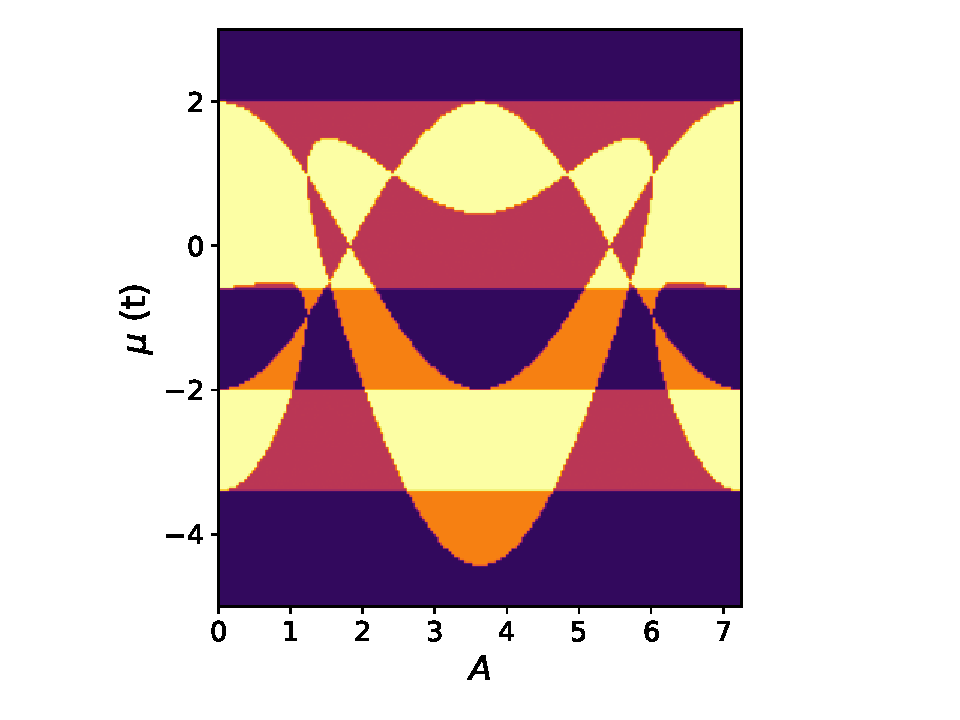
\includegraphics[width=0.50\textwidth]{./figures/supp/topological-phase-diagram-1pi6-n-3.pdf}}
  \hspace{-40pt}
  \subfloat[]{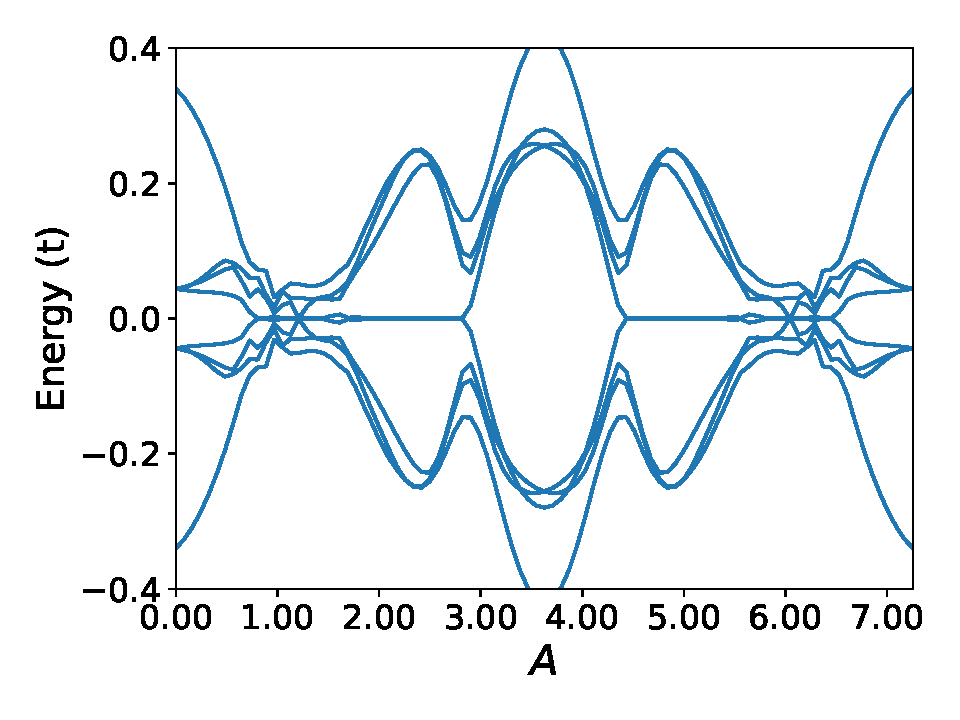
\includegraphics[width=0.50\textwidth]{./figures/supp/spectral-flow-nr-50-w-3-mu-1_6.pdf}} \\
  \hspace{70pt}
  \subfloat[]{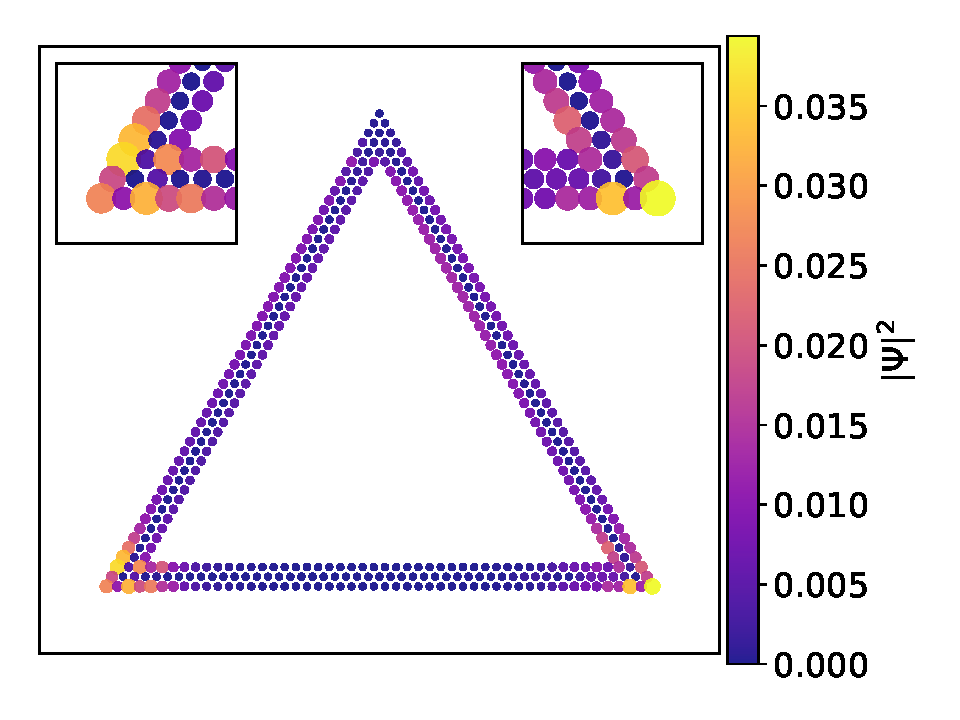
\includegraphics[width=0.50\textwidth]{./figures/supp/GS-A-2_74-nr-50-w-3-mu-1_6.pdf}}
  \caption{(a) Topological phase diagram for a $W=3$ hollow triangle obtained by overlapping the $\mathcal{M}(A, \mu)$ plots of 1D chains with $\mathbf A = A\hat{y}$ and $\mathbf A = A(\frac{\sqrt{      3}}{2}\hat{x}+\frac{1}{2}\hat{y})$. Color scheme: white---$\mathcal{M}=1$, dark blue---$\mathcal{M}=-1$, light blue---$\mathcal{M}=0$ (b) Near-gap BdG eigen-energies vs $A$ for a finite triangle with edge length $L=50$, $W=3$, and $\mu=1.6$. (c) BdG eigenfunction $|\Psi|^2$ summed over the two zero modes at $A=2.4709$.}
  \label{fig: supp pd}
\end{figure}

A model that is closer to a realistic hollow triangular island is the finite-width triangular chain or ribbon. An example, illustrated in Figure \ref{fig: supp pd} (c), has its edge length $L=50$ and width $W=3$. The phase diagram Fig.~\ref{fig: supp pd} (a) is created in a similar way as that in Fig. \ref{fig: pd} (a), assuming a constant vector potential and infinitely long $W=3$ ribbons. The spectral flow for the actual triangle with $\mu = 1.6$ in Fig.~\ref{fig: supp pd} (b) shows MZM in the parameter regions in agreement with the phase diagram. Fig.~\ref{fig: supp pd} (c) plots the MZM wavefunction for $A=2.7409$ and $\mu=1.6$ that are indeed well localized at the bottom corners.

\begin{figure}[!ht]
  \hspace{-20pt}
  \subfloat[]{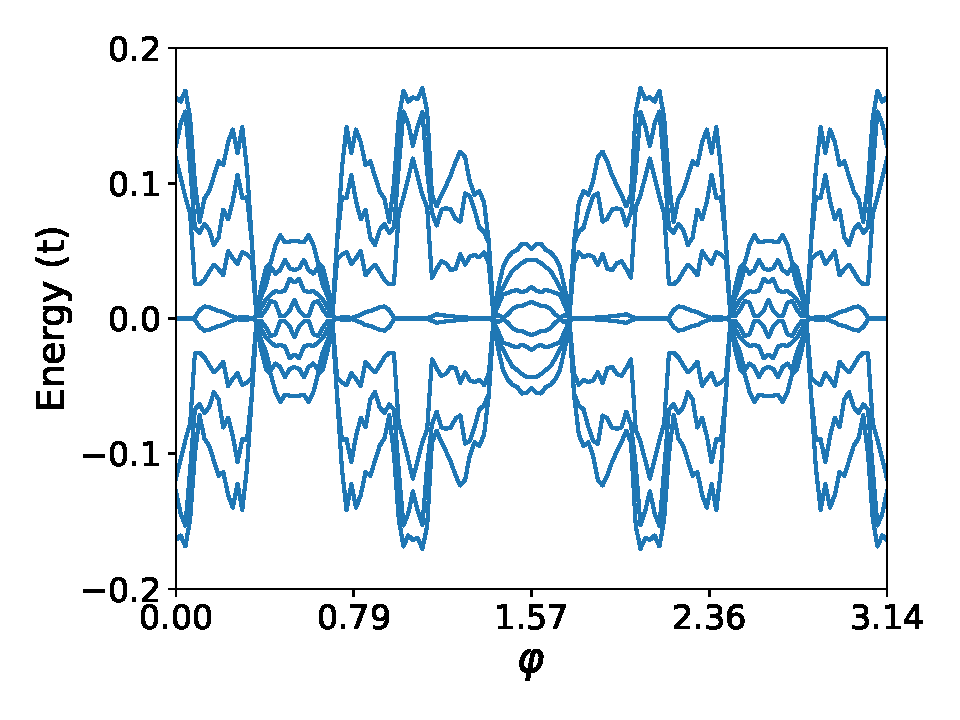
\includegraphics[width=0.5\textwidth]{./figures/supp/spectral-flow-w-3.pdf}}\\
  \subfloat[]{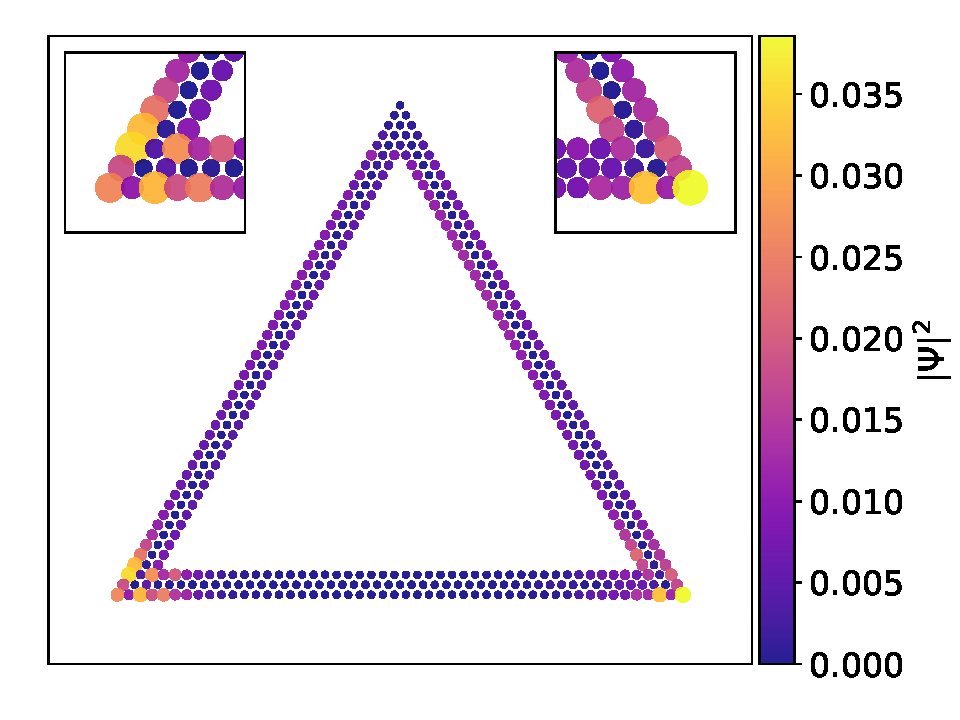
\includegraphics[width=0.4\textwidth]{./figures/supp/GS-T-Square-w-3.pdf}}
  %\subfloat[]{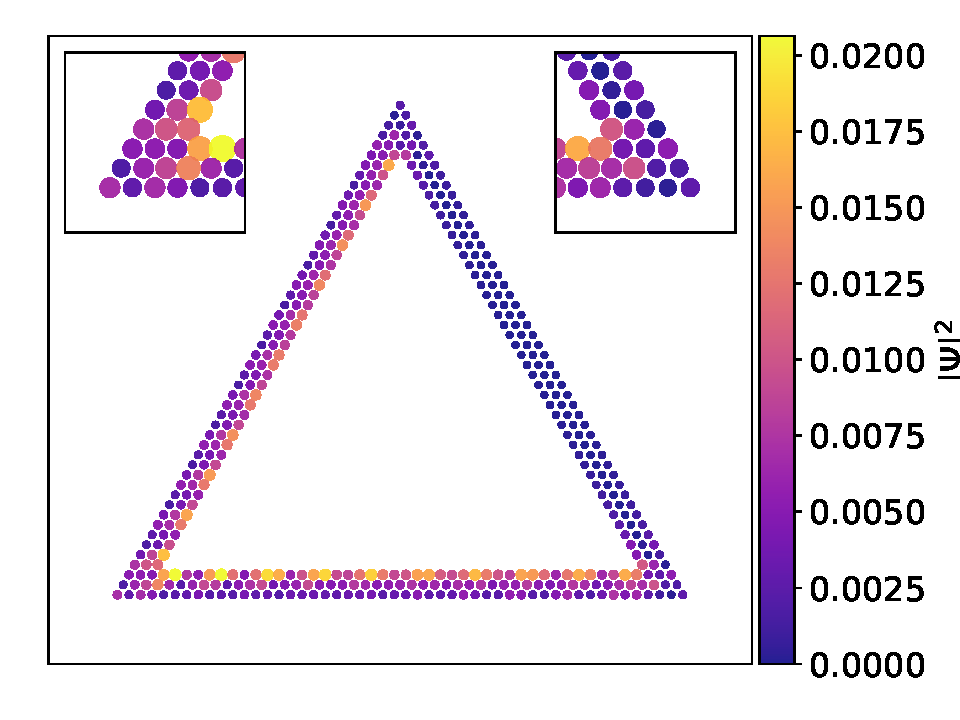
\includegraphics[width=0.4\textwidth]{./figures/supp/GS-T-Circle-w-3.pdf}}
  \subfloat[]{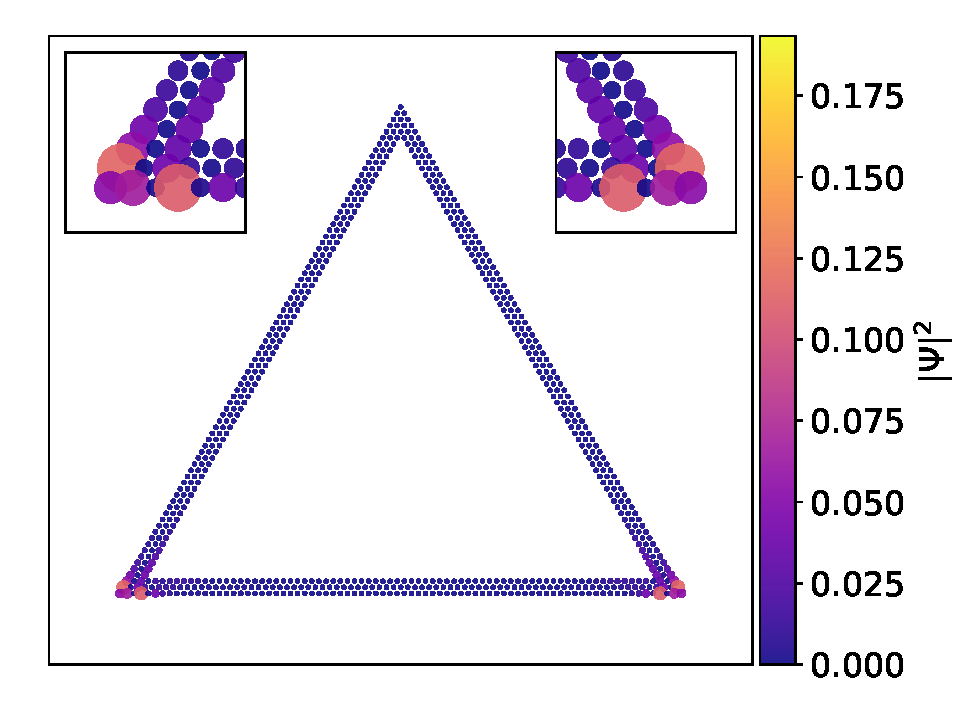
\includegraphics[width=0.4\textwidth]{./figures/supp/GS-T-Diamond-w-3.pdf}}
  \caption{(a) Spectral flow of a hollow triangle with $W=3$, $L=50$, $\mu=1.6$, and $A=2.75$ with increasing rotation angle $\varphi$, defined through $\mathbf A = A(-\sin\varphi \hat{x} + \cos\varphi \hat{y})$. (b-c) BdG eigenfunction $|\Psi|^2$ summed over the two zero modes at $\varphi = 0$ and $\frac{\pi}{3}$, respectively.}
  \label{fig: supp rotation}
\end{figure}

We next rotate the uniform vector potential to examine how the MZM move on a hollow triangle. Figure~\ref{fig: supp rotation} shows the spectral flow and eigenfunctions as we rotate $\varphi=0$ to $\varphi=\pi$ counterclockwisely. The two MZM cycle through the three vertices in a similar manner as that in Fig.~4 of the main text (only the MZM wavefunctions at $\varphi = 0$ and $\frac{\pi}{3}$ are plotted as representatives of the $\varphi = n\pi/3$ cases). Note that the spectral flow has 3-fold rotation symmetry but not 6-fold, since increasing $\varphi$ by $\frac{2\pi}{3}$ is equivalent to rotating the coordinate system clockwisely by $\frac{2\pi}{3}$. In contrast, rotating the vector potential by $\frac{\pi}{3}$, if without an additional sign change of the $p$-wave pairing potential, is not an exact symmetry of the finite triangle. Also we did not try to scrutinize the phase diagram to find a parameter path in which the bulk gap does not close, as in the $W=1$ case in the main text. Here we just point out that identifying a system-specific parameter path for adiabatic manipulation of MZM is in principle always possible, especially if one is allowed to have more knobs other than $\varphi$ in real structures, such as tuning the chemical potential of individual edges or the size of the vector potential, etc.

\section{Braiding MZM in a small network of triangles}

\begin{figure}[!ht]
  \hspace{-30pt}
  \subfloat[]{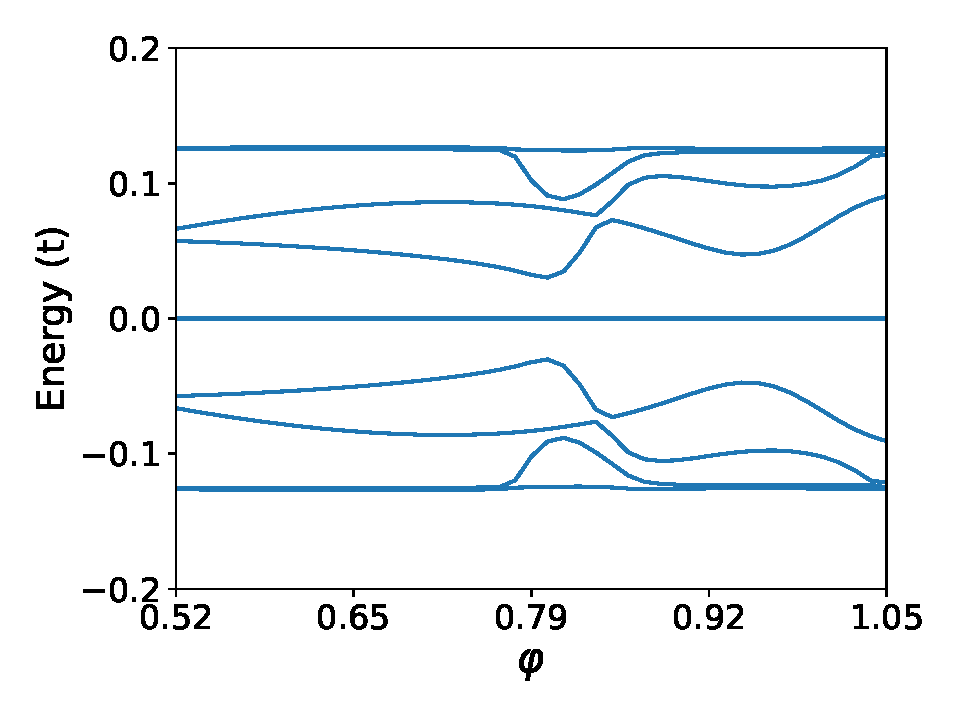
\includegraphics[width=0.4\textwidth]{./figures/supp/spectral-flow-braiding.pdf}} \\
  \vspace{-10pt}
  \subfloat[]{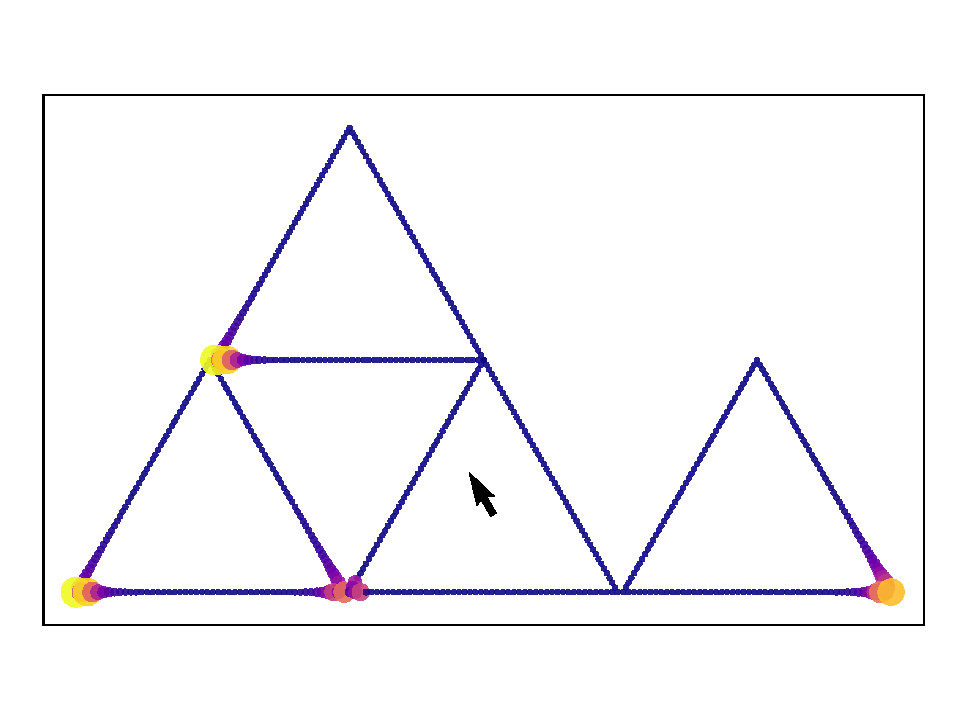
\includegraphics[width=0.30\textwidth]{./figures/supp/GS-T-0_5236.pdf}}
  \subfloat[]{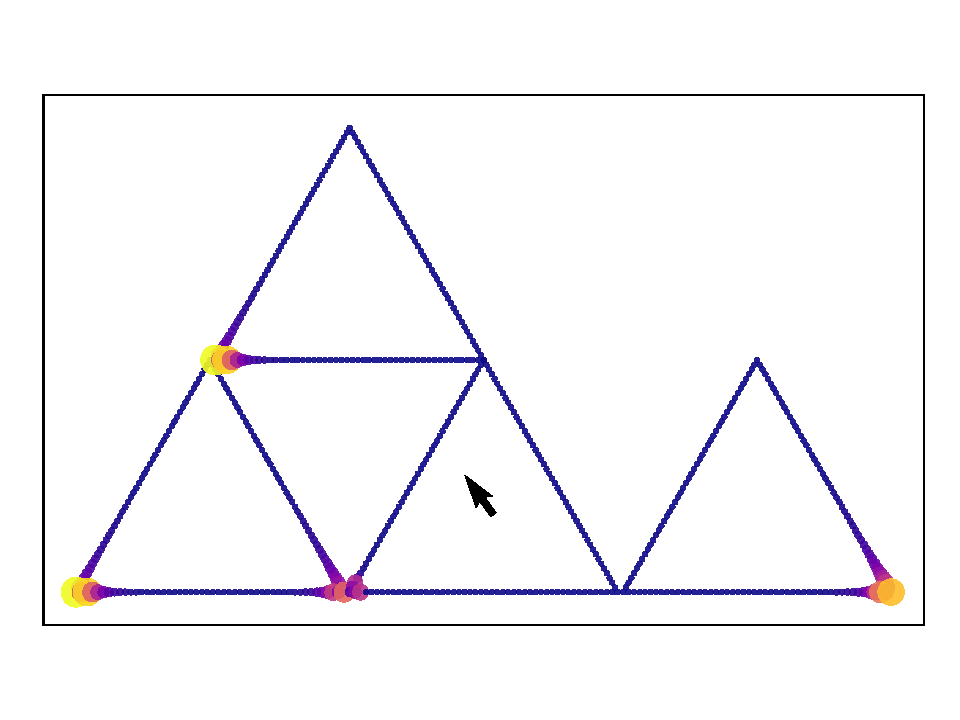
\includegraphics[width=0.30\textwidth]{./figures/supp/GS-T-0_6283.pdf}}
  \subfloat[]{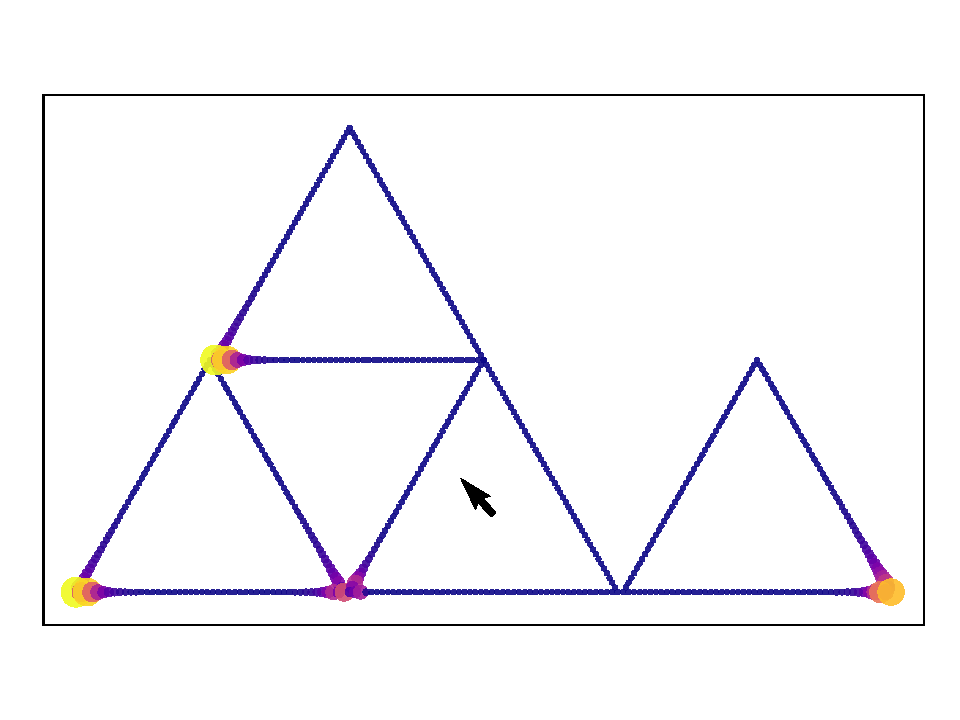
\includegraphics[width=0.30\textwidth]{./figures/supp/GS-T-0_7330.pdf}} \\
  \subfloat[]{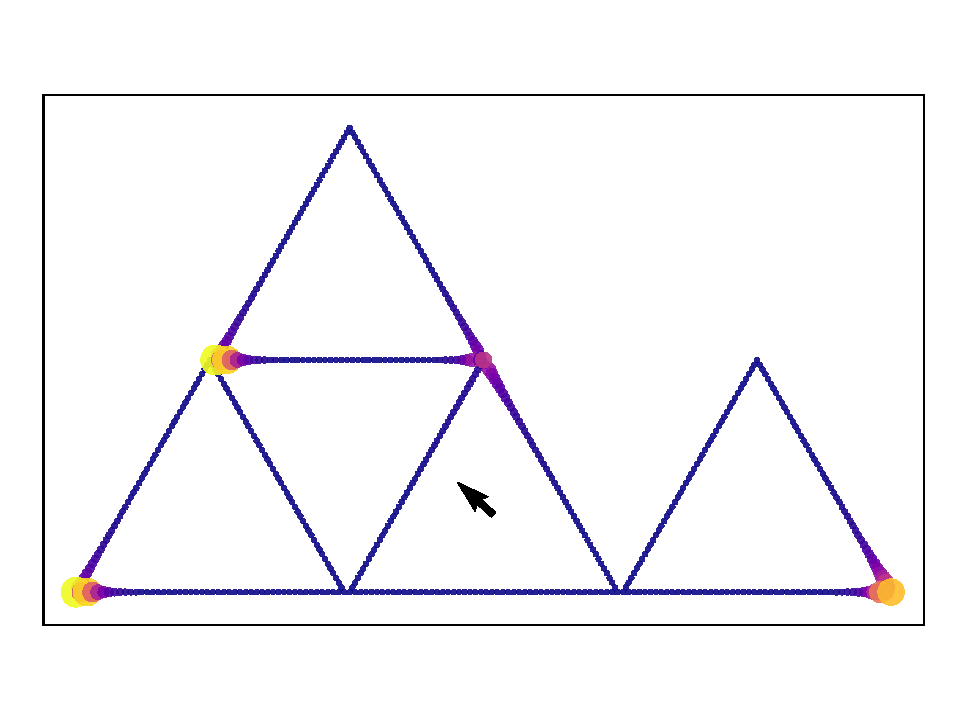
\includegraphics[width=0.30\textwidth]{./figures/supp/GS-T-0_8378.pdf}}
  \vspace{-10pt}
  \subfloat[]{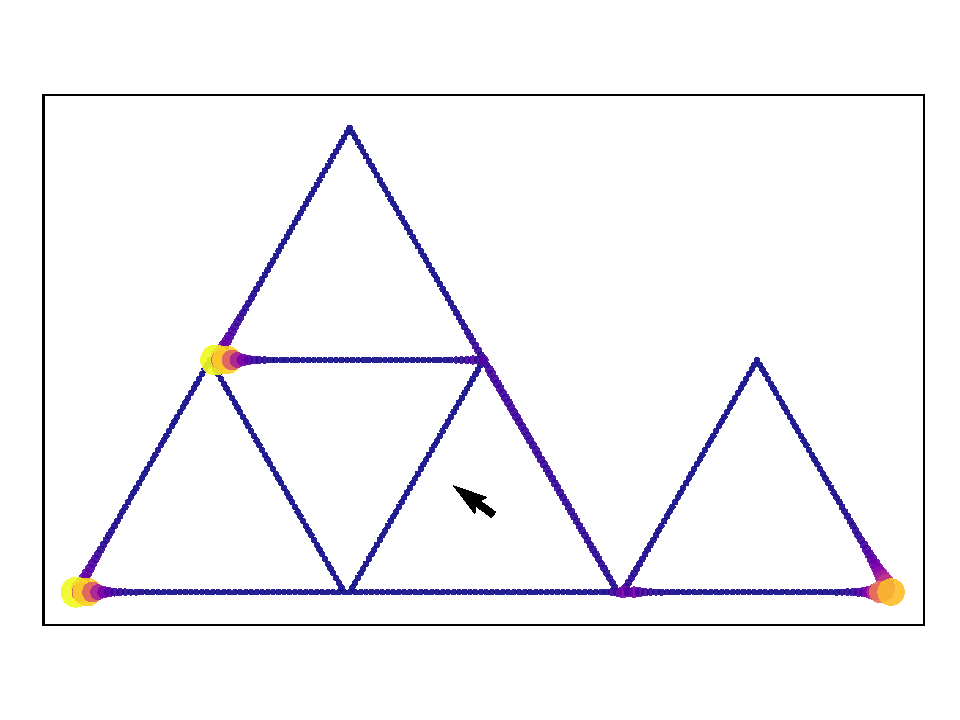
\includegraphics[width=0.30\textwidth]{./figures/supp/GS-T-0_9425.pdf}}
  \subfloat[]{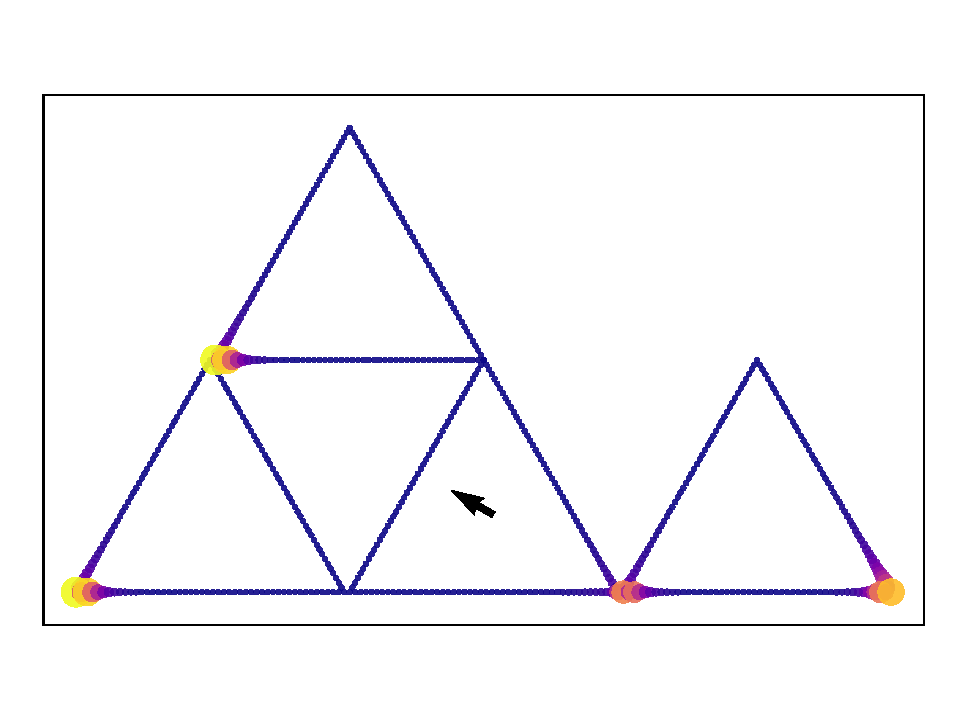
\includegraphics[width=0.30\textwidth]{./figures/supp/GS-T-1_0472.pdf}}
  \caption{(a) Spectral flow for the critical step of swapping $\gamma_2$ and $\gamma_3$ in the example of Fig.~5 in the main text, calculated using four corner-sharing triangles of $W=1$ and $L=50$, with $\mu=1.6$ and $A=2.6$. Vector potential for the middle triangle in the bottom row can rotate according to $\mathbf A = A(-\sin\varphi \hat{x} + \cos\varphi \hat{y})$ from $\varphi = \frac{\pi}{6}$ to $\frac{\pi}{3}$, while the other three have fixed $\varphi = 0$. (b)-(g) BdG eigenfunction $|\Psi|^2$ summed over the four zero modes at equally-spaced points along the rotation path. The black arrow indicates the direction of the vector potential for the bottom middle triangle.}\label{fig: supp braiding}
\end{figure}

In this section we show that one can braid two out of four MZM, a minimal setting for nontrivial manipulation of the degenerate many-body ground states, by using a small network of corner-sharing triangles. We focus on the critical step of swapping $\gamma_2$ and $\gamma_3$ as labeled in Fig.~5 of the main text. This can be done by rotating the vector potential of the triangle in the middle of the bottom row from $\varphi = \frac{\pi}{6}$ to $\frac{\pi}{3}$. More specifically, when $\varphi = \frac{\pi}{6}$, with the chosen values of $\mu$ and $A$, only the right edge of the said triangle is topologically nontrivial. The chain that hosts $\gamma_{3,4}$ thus extends through this nontrivial edge to the top triangle as in Fig.~\ref{fig: supp braiding} (b). On the other hand, when $\varphi$ increases to $\frac{\pi}{3}$, the nontrivial edge of the middle triangle changes from right to left, which leads to $\gamma_2$ hopping from its left corner to the right through the top corner, while $\gamma_3$ is unaffected [Figs.~\ref{fig: supp braiding} (c-g)]. As a result the $\gamma_2,\gamma_3$ swapping is done without closing the bulk gap, as can be seen from the spectral flow in Fig.~\ref{fig: supp braiding} (a).


\section{Additional results using inhomogeneous vector fields}

While we have showed a constant vector field works to induce and manipulate MZM for a triangular chain and hollow triangle it remains to be seen if inhomogeneous vector potential fields can repoduce the same results. We expect this to be the case due to the topological phase diagram seen in \ref{fig: pd} (a) and \ref{fig: supp pd} (a) and the results that followed for a constant vector potential.

\begin{figure}[!ht]
  \subfloat[]{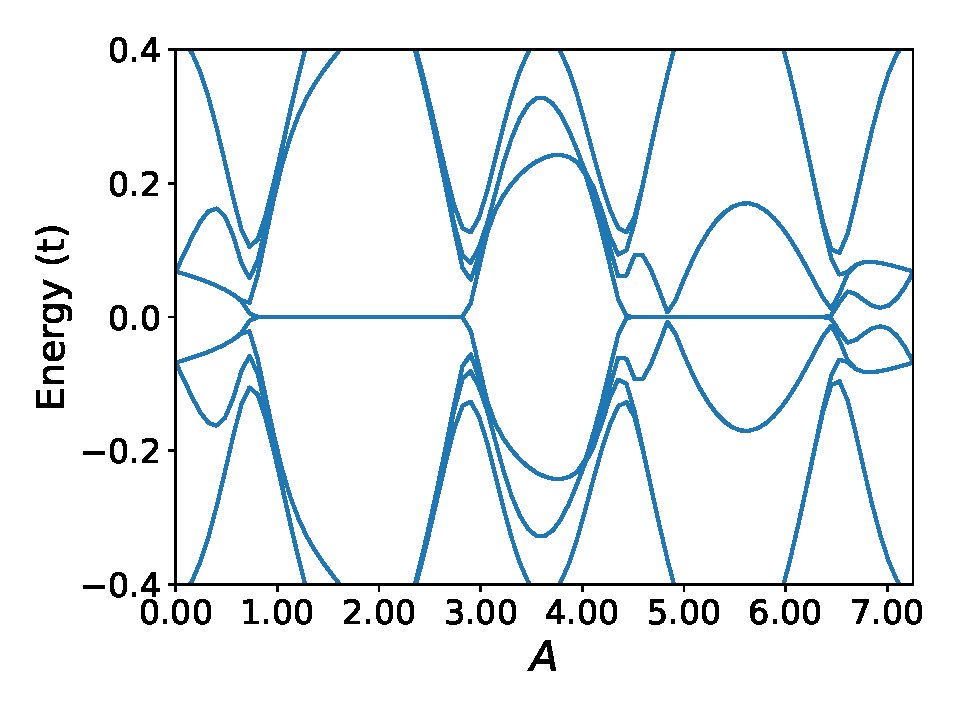
\includegraphics[width=0.5\textwidth]{./figures/spectral-flow-heaviside-w-1-mu-1_6.pdf}}
  \subfloat[]{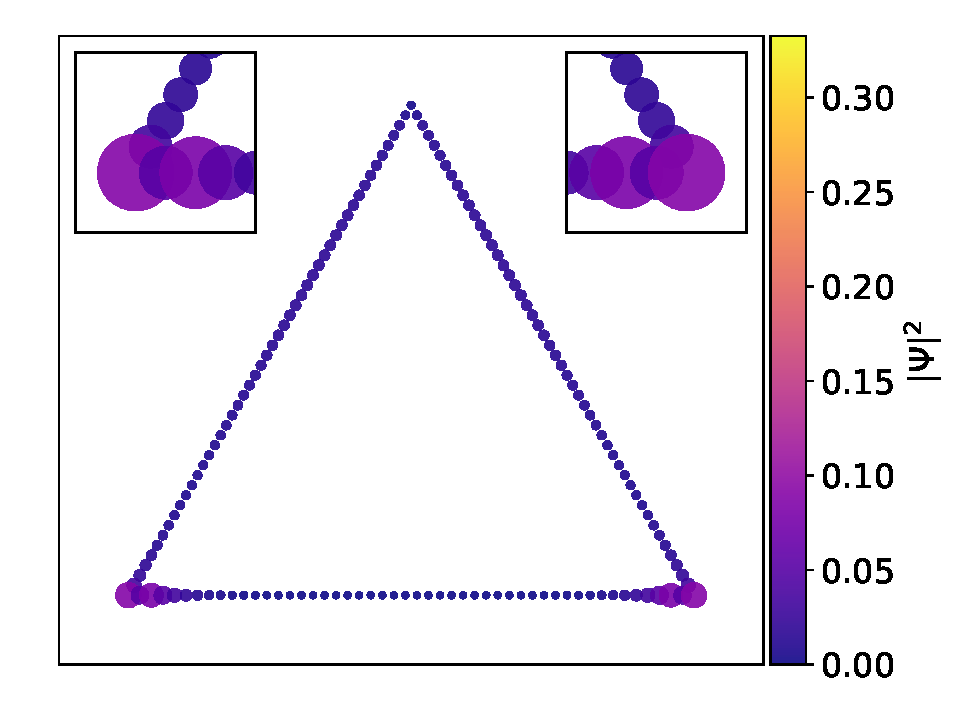
\includegraphics[width=0.5\textwidth]{./figures/GS-A-2_7409-heaviside-w-1-mu-1_6.pdf}}
  \caption{(a) Spectral flow of a hollow triangle with $W=1$, $L=50$, and $\mu=1.6$ for increasing heaviside vector potential strength defined by $\vec{A} = A [1-2\Theta(x)] \hat{y}$ (b) BdG eigenfunction $|\Psi|^2$ summed over the two zero modes at $A = 2.7409$.}
  \label{fig: heaviside-increasing-w-1}
\end{figure}

\begin{figure}[!ht]
  \subfloat[]{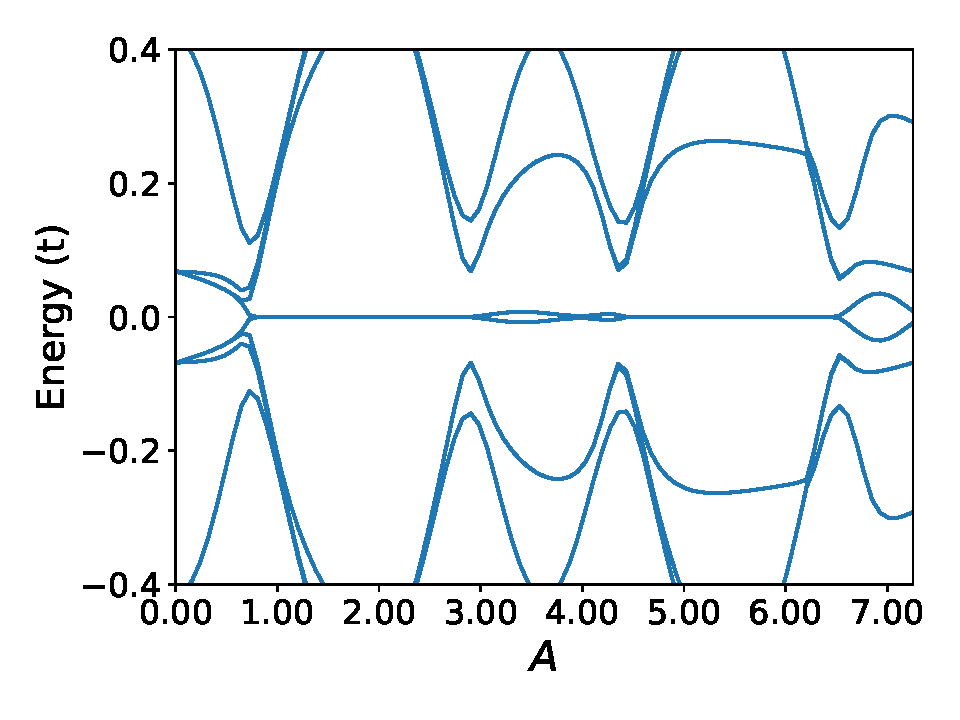
\includegraphics[width=0.5\textwidth]{./figures/spectral-flow-tanh-w-1-mu-1_6.pdf}}
  \subfloat[]{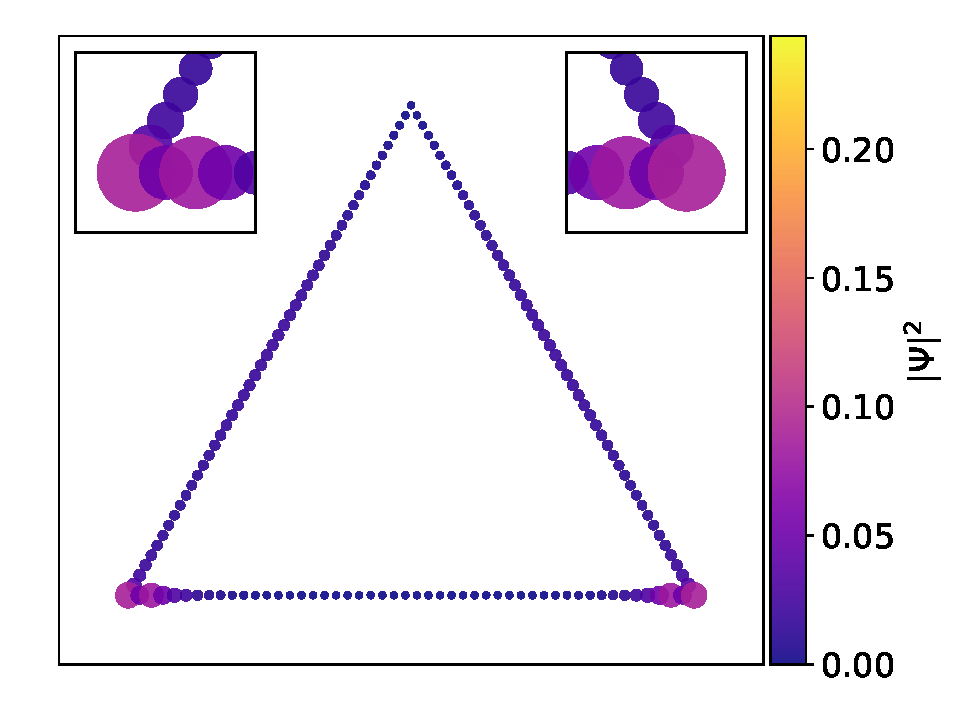
\includegraphics[width=0.5\textwidth]{./figures/GS-A-2_7409-tanh-w-1-mu-1_6.pdf}}
  \caption{(a) Spectral flow of a hollow triangle with $W=1$, $L=50$, and $\mu=1.6$ for increasing tanh vector potential strength defined by $\vec{A} = -A \tanh(x/2w)\hat{y}$, $w=a/2$ (b) BdG eigenfunction $|\Psi|^2$ summed over the two zero modes at $A = 2.7409$.}
  \label{fig: tanh-increasing-w-1}
\end{figure}

For hollow triangle of width, $W=1$ subject to a heaviside vector potential we see a similar spectral flow and MZM in Fig. \ref{fig: heaviside-increasing-w-1} to match \ref{fig: pd}.
If the heaviside vector potential is not so easily made in lab it may be easier to model a tanh function instead.
Also, in the limit that the tanh's function width, $w$, goes to zero it is equivalent to the heaviside function.
A tanh vector potential can match the same results as seen in Fig. \ref{fig: tanh-increasing-w-1}.
It should be mentioned that the width of the tanh function should be on the order or smaller than the distance between to neighboring lattice points, if two neighboring sites overall phase accumulation is not large enough to match the topological phase diagram then the bulk edge correspondence at the tanh's inflection point would cause additional MZM to appear.
In other words, the top edges of the triangle should be one long bent trivial edge but if the tanh's width is too large the two edges become separated by a small non-trivial topological corner-edge because the Peierls phase is too small.
Increasing the width of the hollow triangle to $W=3$, we see similar results for heaviside, Fig. \ref{fig: heaviside-increasing-w-3}, and tanh, Fig. \ref{fig: tanh-increasing-w-3}, compared to a constant vector potnential, Fig. \ref{fig: supp pd}.

\begin{figure}[!ht]
  \subfloat[]{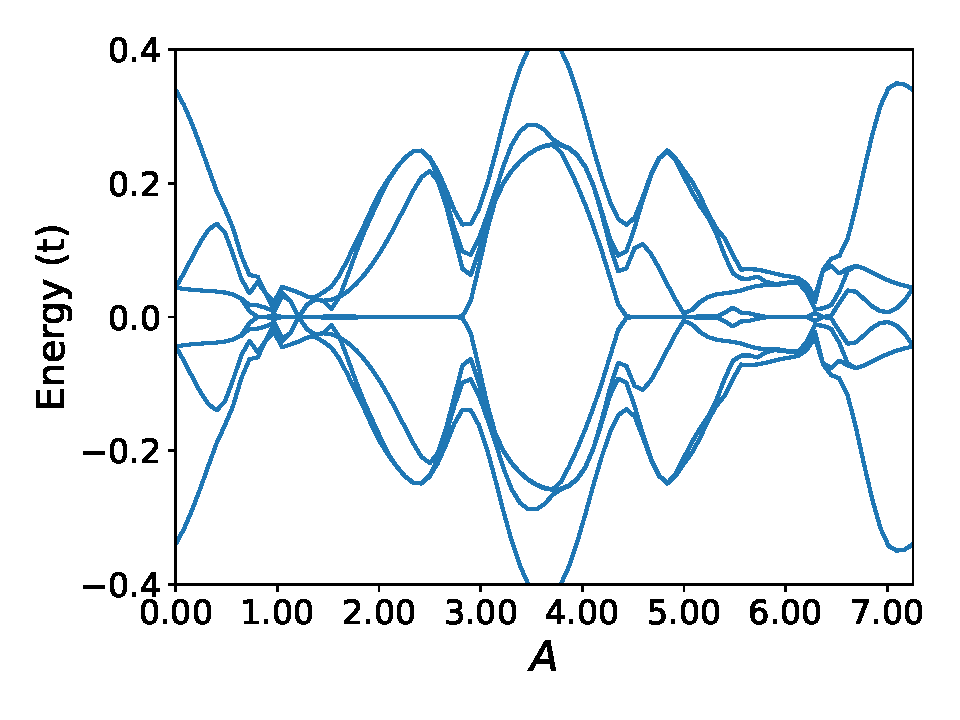
\includegraphics[width=0.5\textwidth]{./figures/spectral-flow-heaviside-w-3-mu-1_6.pdf}}
  \subfloat[]{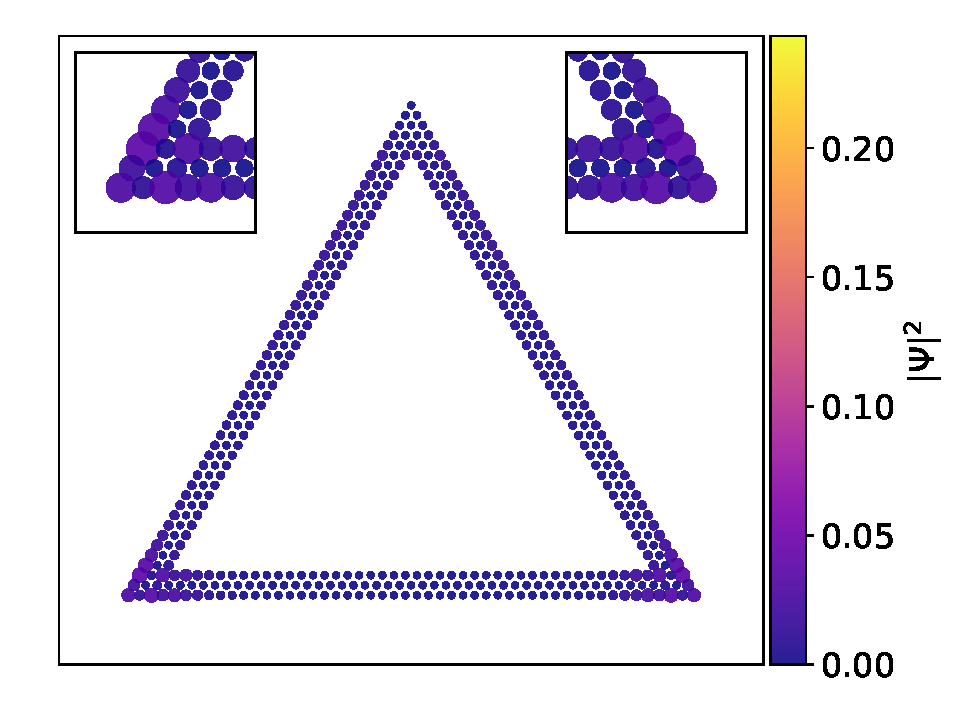
\includegraphics[width=0.5\textwidth]{./figures/GS-A-2_7409-heaviside-w-3-mu-1_6.pdf}}
  \caption{(a) Spectral flow of a hollow triangle with $W=3$, $L=50$, and $\mu=1.6$ for increasing heaviside vector potential strength defined by $\vec{A} = A [1-2\Theta(x)] \hat{y}$ (b) BdG eigenfunction $|\Psi|^2$ summed over the two zero modes at $A = 2.7409$.}
  \label{fig: heaviside-increasing-w-3}
\end{figure}

\begin{figure}[!ht]
  \subfloat[]{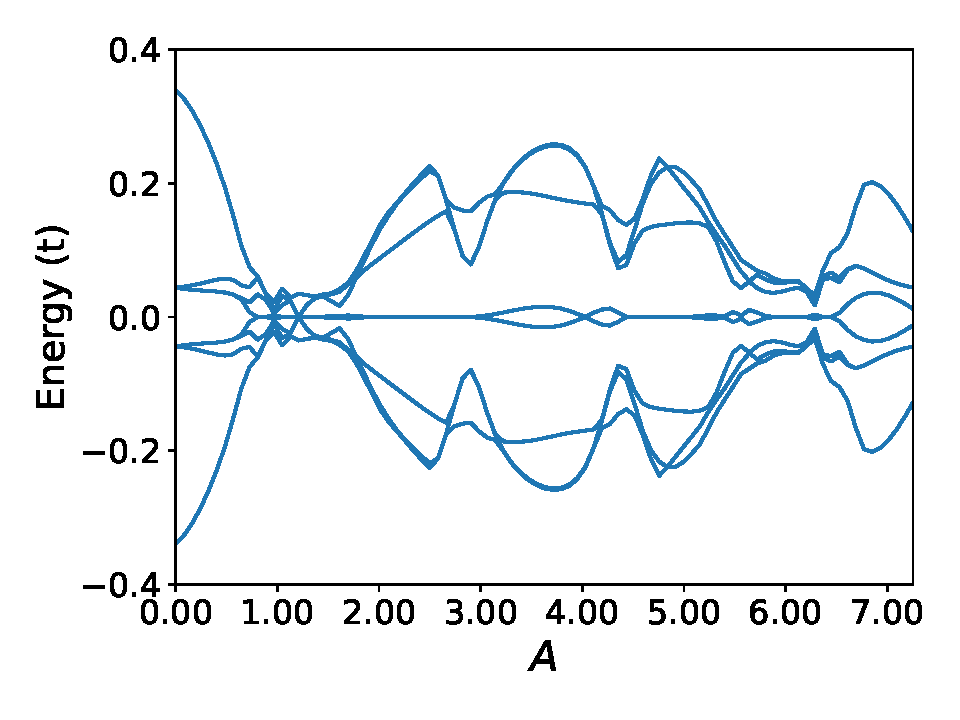
\includegraphics[width=0.5\textwidth]{./figures/spectral-flow-tanh-w-3-mu-1_6.pdf}}
  \subfloat[]{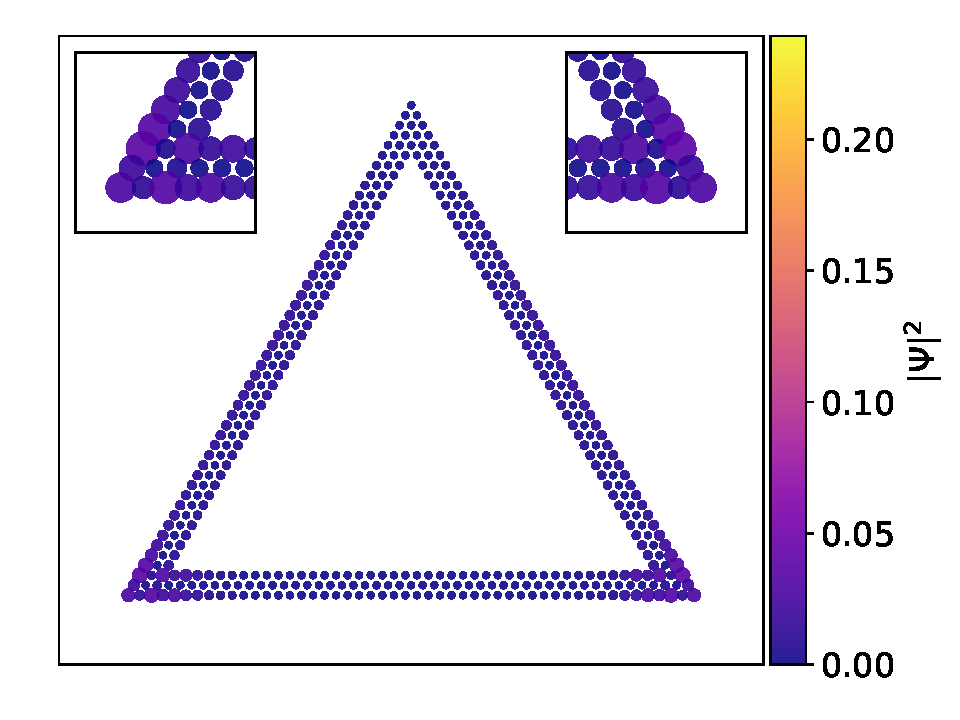
\includegraphics[width=0.5\textwidth]{./figures/GS-A-2_7409-tanh-w-3-mu-1_6.pdf}}
  \caption{(a) Spectral flow of a hollow triangle with $W=3$, $L=50$, and $\mu=1.6$ for increasing tanh vector potential strength defined by $\vec{A} = -A \tanh(x / 2w)\hat{y}$, $w=a/2$ (b) BdG eigenfunction $|\Psi|^2$ summed over the two zero modes at $A = 2.7409$.}
  \label{fig: tanh-increasing-w-3}
\end{figure}


We look at a linear vector potential next.
A topological phase diagram for a linear vector potential is possible to compute, however, it requires a lattice space matrix instead of momentum space matrix due to having no periodic boundary conditions.
It also requires separate calculations for longer traingular lattice ribbons.
Computation times can become unruly when modeling large triangles for a high density phase diagram of $A$ and $\mu$ values.
We could, however, use the topological phase diagram in Fig. \ref{fig: pd} to guess the topology for the varying Peierls phases along an edge.
Fig. \ref{fig: linear-increasing} shows some critical points for MZMs to appear with $\mu=0$ for a hollow triangle of $W=1$ and $W=3$, respectively.
Fig. \ref{fig: linear-increasing-mu-1_6} shows apparent zero modes for a range of $A$ values for a hollow triangle of $W=1$ and $W=3$, respectively.
For similar reasons why the tanh function width needs to be small, it may be difficult to have the upper parts of the triangles top edges be all trivial topology, a small section may centered on the top corner may be non-trivial, thus hosting additional MZMs, as seen in Fig. \ref{fig: linear-increasing-mu-1_6} (c-d) half way up the triangles.

\begin{figure}[!ht]
  \subfloat[]{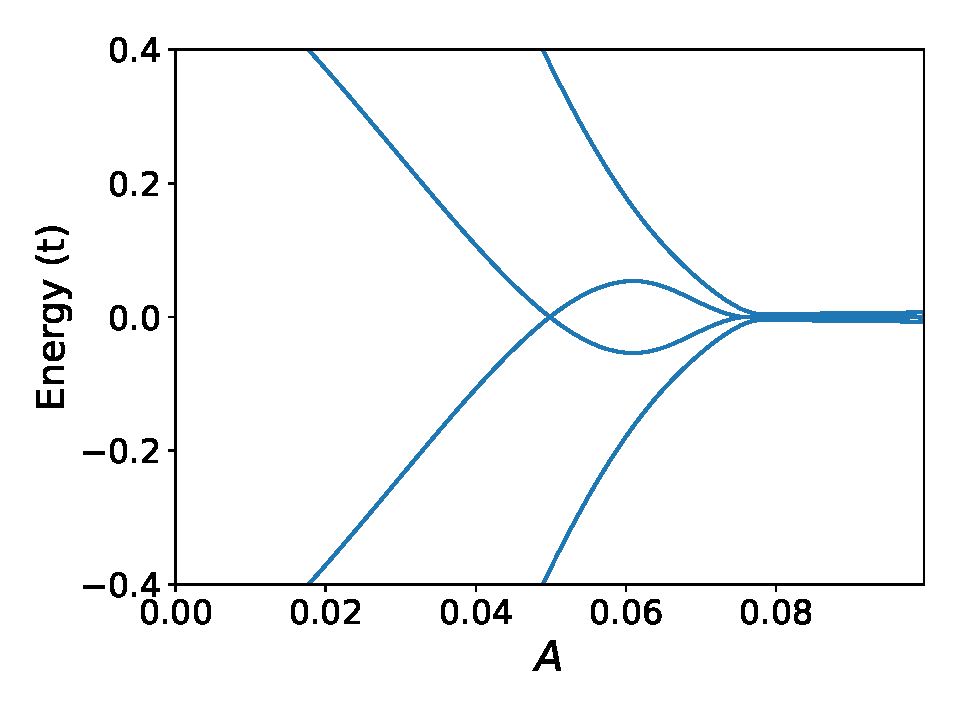
\includegraphics[width=0.5\textwidth]{./figures/spectral-flow-linear-w-1-mu-0.pdf}}
  \subfloat[]{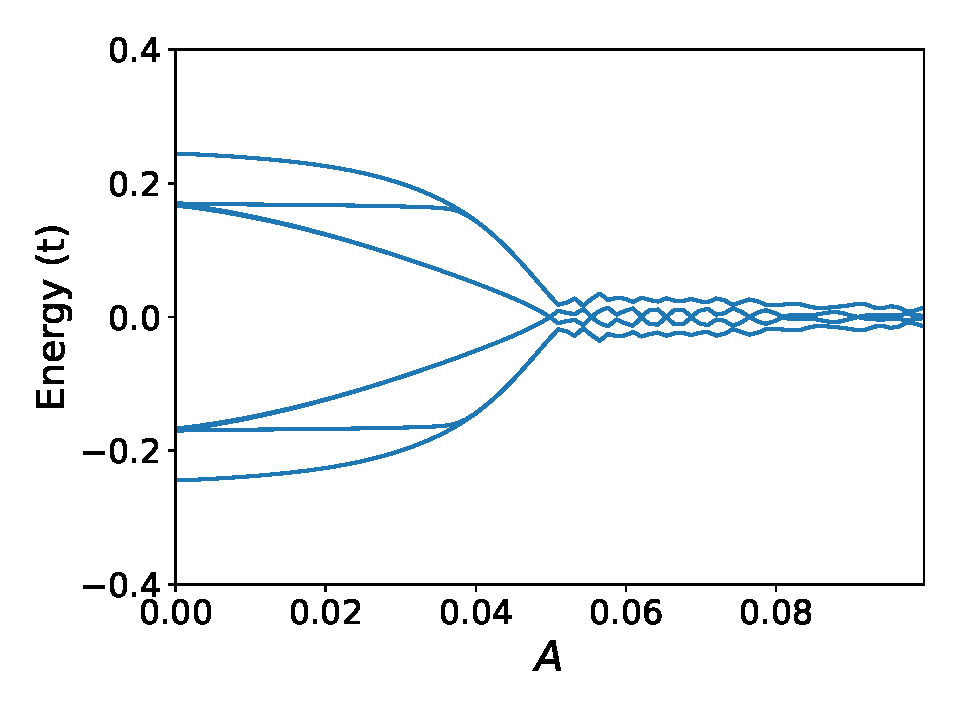
\includegraphics[width=0.5\textwidth]{./figures/spectral-flow-linear-w-3-mu-0.pdf}}\\
  \subfloat[]{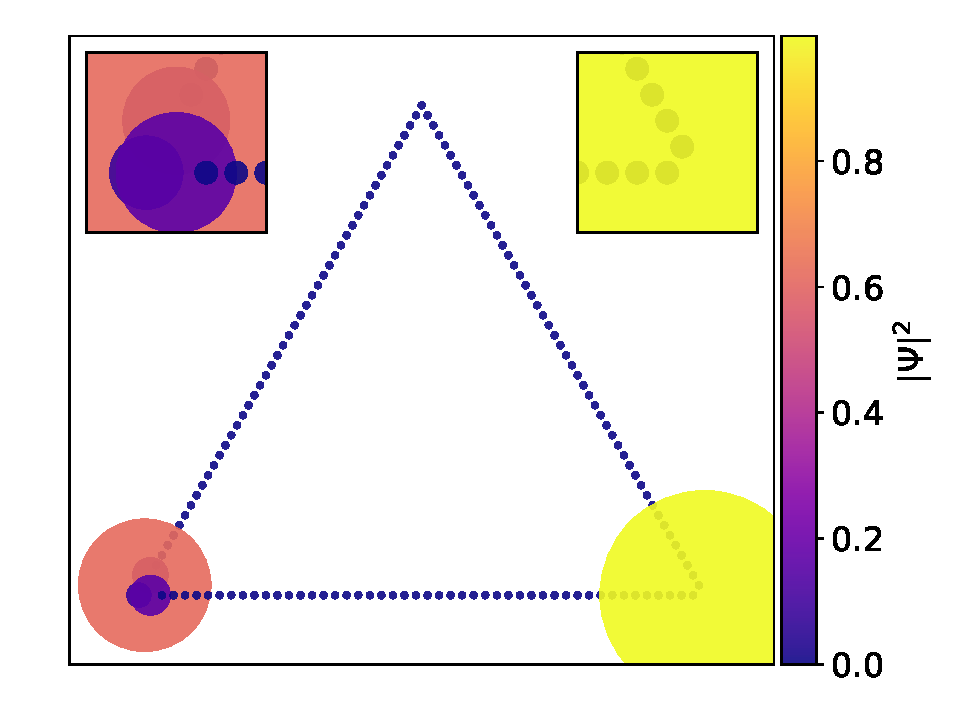
\includegraphics[width=0.5\textwidth]{./figures/GS-A-0_0499-linear-w-1-mu-0.pdf}}
  \subfloat[]{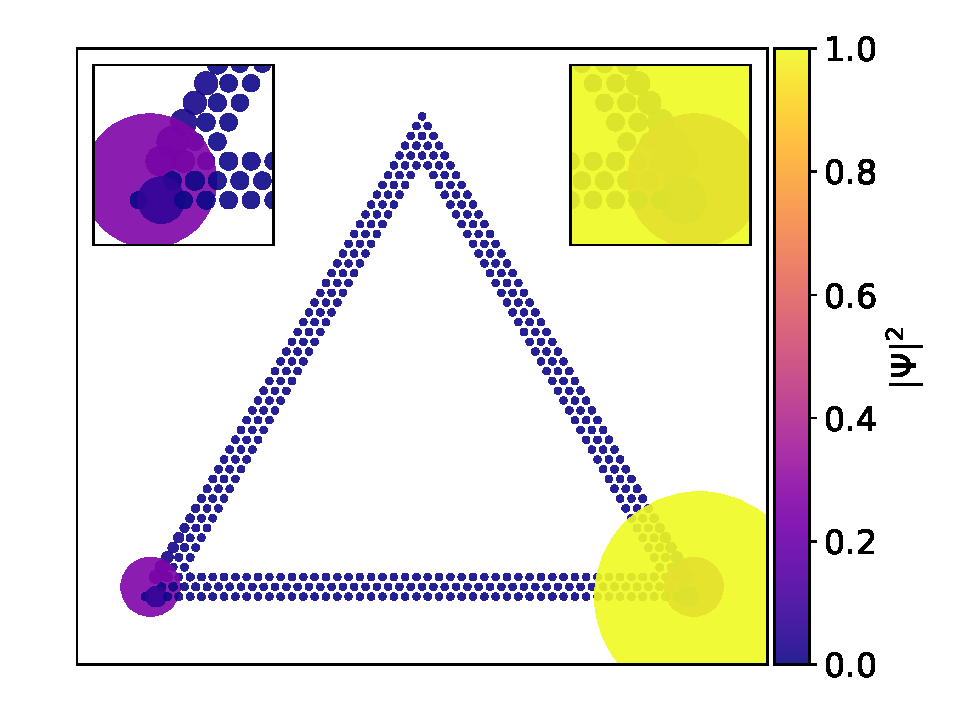
\includegraphics[width=0.5\textwidth]{./figures/GS-A-0_0499-linear-w-3-mu-0.pdf}}
  \caption{Spectral flow of a hollow triangle with $L=50$, and $\mu=0$ for increasing linear vector potential strength defined by $\vec{A} = -Ax\hat{y}$ (a) $W=1$ and (b) $W=3$ (c-d) Wavefunctions of the MZM at $A=0.0499$ for both widths, respectively.}
  \label{fig: linear-increasing}
\end{figure}

\begin{figure}[!ht]
  \subfloat[]{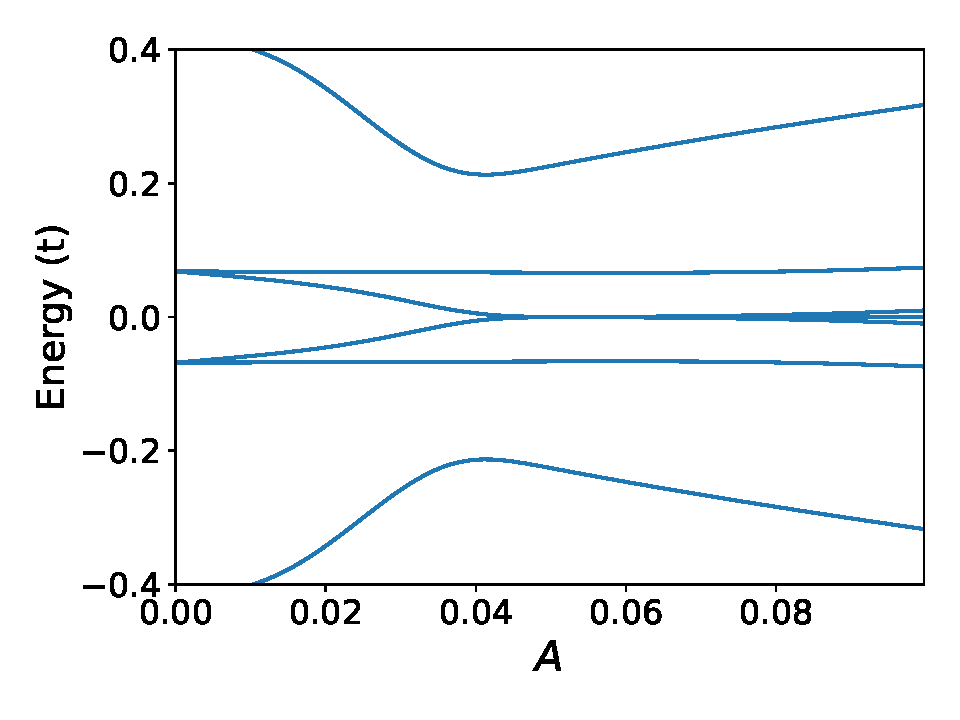
\includegraphics[width=0.5\textwidth]{./figures/spectral-flow-linear-w-1-mu-1_6.pdf}}
  \subfloat[]{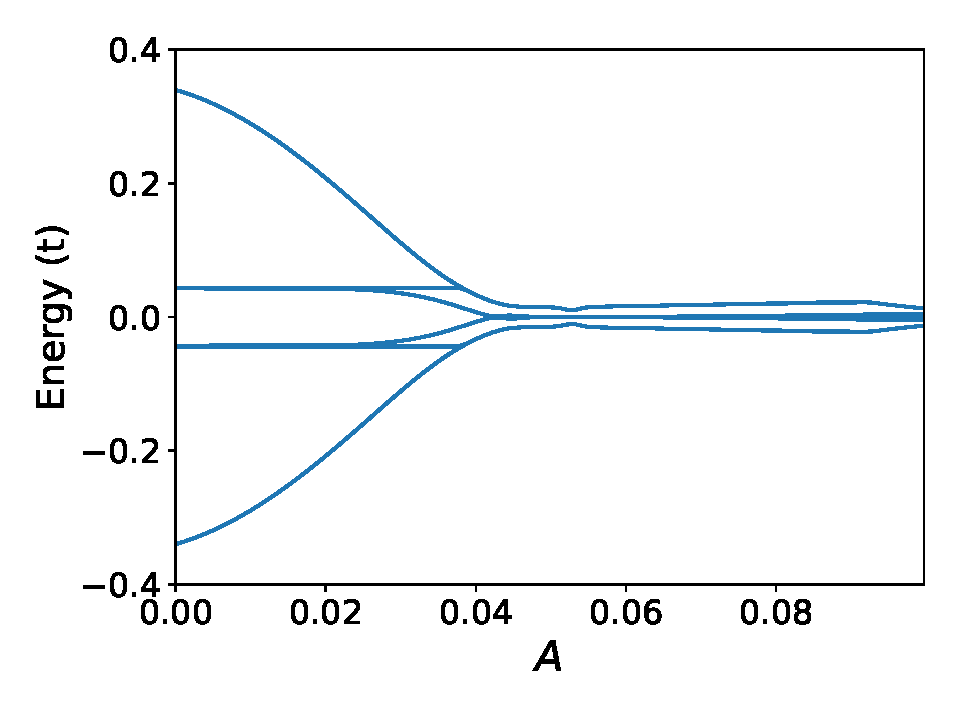
\includegraphics[width=0.5\textwidth]{./figures/spectral-flow-linear-w-3-mu-1_6.pdf}}\\
  \subfloat[]{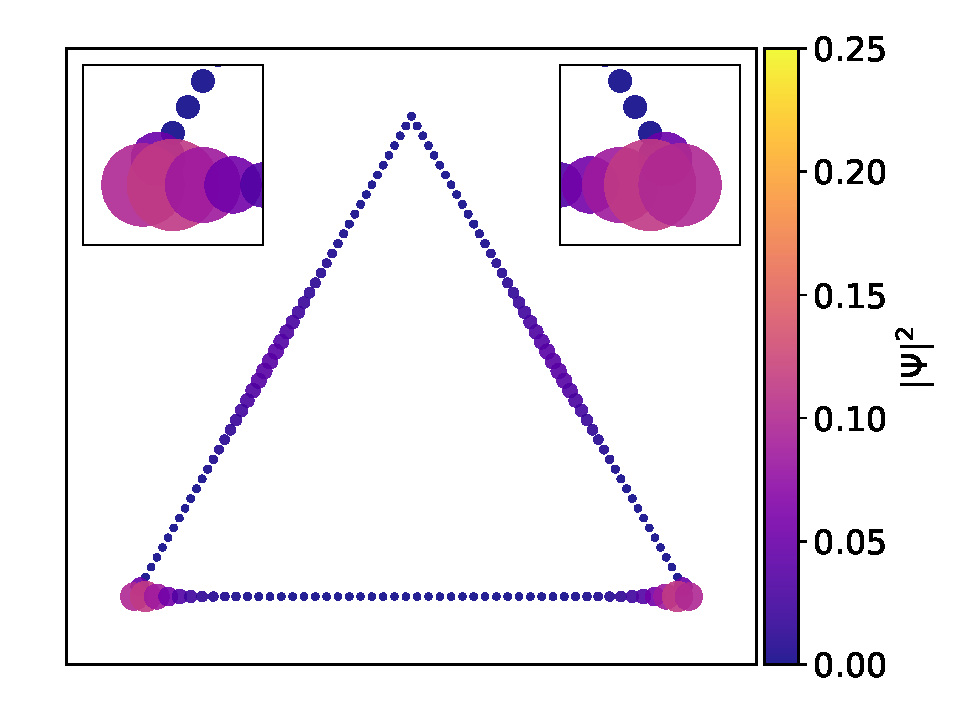
\includegraphics[width=0.5\textwidth]{./figures/GS-A-0_0598-linear-w-1-mu-1_6.pdf}}
  \subfloat[]{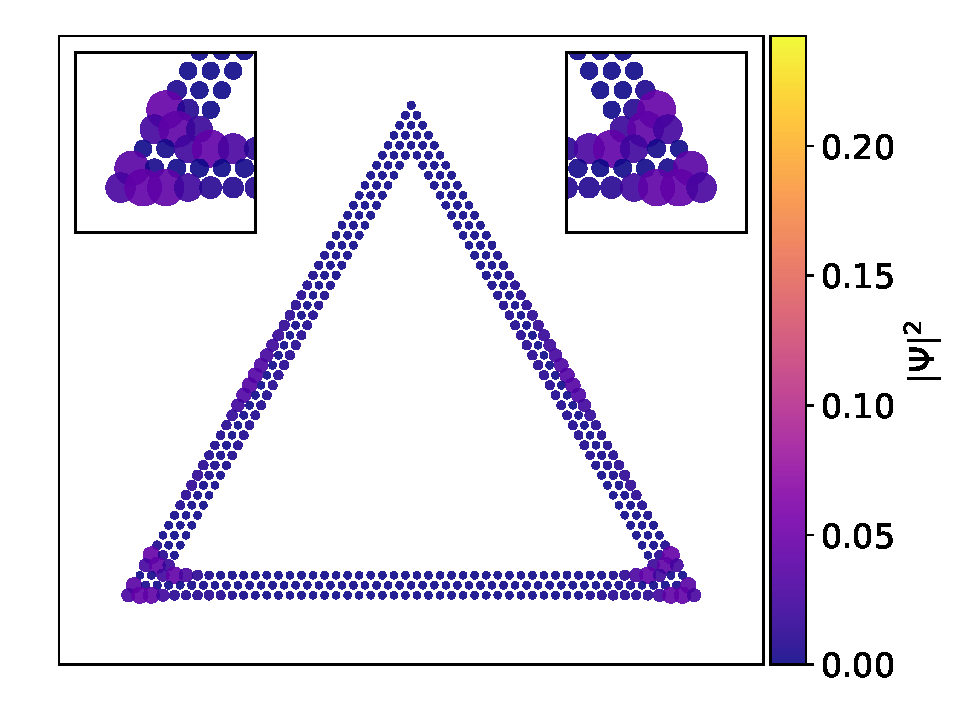
\includegraphics[width=0.5\textwidth]{./figures/GS-A-0_0598-linear-w-3-mu-1_6.pdf}}
  \caption{Spectral flow of a hollow triangle with $L=50$, and $\mu=1.6$ for increasing linear vector potential strength defined by $\vec{A} = -Ax\hat{y}$ (a) $W=1$ and (b) $W=3$. (c-d) Wavefunctions of the MZM at $A=0.0598$ for both widths, respectively.}
  \label{fig: linear-increasing-mu-1_6}
\end{figure}

